\chapter{ANOVA}
\label{ch-ANOVA}

ANOVA 
stands for \qt{Analysis of Variance}.

\section{Law of Total Variance}

\begin{claim}
(Law of Total Variance)
Suppose $P:S_\rvx\times S_\rvy\rarrow [0,1]$
is a probability distribution.
Suppose $f:S_\rvx\times S_\rvy\rarrow \RR$
 and $f=f(x,y)$. Then
\beq
Var_{\rvx, \rvy}(f)=
E_\rvy[Var_{\rvx|\rvy}(f)]
+
Var_\rvy(E_{\rvx|\rvy}[f])
\;.
\eeq
In particular,
\beq
Var_{\rvx}(x)=
E_\rvy[Var_{\rvx|\rvy}(x)]
+
Var_\rvy(E_{\rvx|\rvy}[x])
\;.
\eeq

\end{claim}
\proof

Let
\beq
A=\sum_y P(y)\left(\sum_x P(x|y)f\right)^2
\;.
\eeq
Then

\beqa
Var_{\rvx, \rvy}(f)&=& \sum_{x,y}P(x,y)f^2 -
\left( \sum_{x,y} P(x,y) f\right)^2
\\
&=&
\left\{
\begin{array}{l}
\sum_{x,y}P(x,y)f^2
-A
\\
+\left(A-\left( \sum_{x,y} P(x,y) f\right)^2\right)
\end{array}
\right.
\eeqa

\beqa
E_\rvy[Var_{\rvx|\rvy}(f)]
&=&
\sum_y P(y)\left(\sum_x P(x|y)f^2
-
\left(\sum_x P(x|y)f\right)^2
\right)
\\
&=&
\sum_{x,y}P(x,y)f^2
-A
\eeqa

\beqa
Var_\rvy(E_{\rvx|\rvy}[f])
&=&
\sum_y P(y)
\left(\sum_x P(x|y)f\right)^2
-\left(
\sum_y P(y)\sum_xP(x|y)f
\right)^2
\\
&=&
A-\left( \sum_{x,y} P(x,y) f\right)^2
\eeqa
\qed

\section{Sum of Squares Estimates}
Consider 
a population $\Sigma$
partitioned 
into groups $\Sigma_g$
such that
$\Sigma=\cup_{g=1}^{ng}\Sigma_g$,
where the 
$\Sigma_g$ are mutually disjoint.

Let

$dof$ stand for
\qt{degrees of freedom}

$SS$ stand for \qt{Sum of Squares}

$MS$ stand for \qt{Mean Square}

$x_{\Sigma_g}=
\{x_{\s|g}\}_{\s\in\Sigma_g}$

Define the total 
and group mean values by

\beq
\ol{x}=\frac{1}{|\Sigma|}
\sum_{g=1}^{ng}\sum_{\s\in\Sigma_g}
x_{\s|g}
\eeq

\beq
\ol{x}_g=\frac{1}{|\Sigma_g|}
\sum_{\s\in\Sigma_g}
x_{\s|g}
\eeq

Define the {\bf SS Total} by
\beqa
SS_T
&=&\sum_{g=1}^{ng}\sum_{\s\in\Sigma_g}
(x_{\s|g}- \ol{x})^2
\\
&=&
|\Sigma| Var_{\rvx}(x)
\eeqa
with $dof$ and $MS$ given by

\beq
dof_T=|\Sigma|-1
,\;
MS_T=\frac{SS_T}{dof_T}
\eeq

Define the {\bf SS Within} by

\beqa
SS_W &=& \sum_{g=1}^{ng}
\sum_{\s\in\Sigma_g}(x_{\s|g}- \ol{x}_g)^2
\\
&=&|\Sigma|
\sum_{g=1}^{ng}
\frac{|\Sigma_g|}{|\Sigma|}
\left\{
\frac{1}{|\Sigma_g|}
\sum_{\s\in\Sigma_g}
(x_{\s|g}- \ol{x}_g)^2
\right\}
\\
&=&
|\Sigma|
E_\rvg[
Var_{\rvx|\rvg}(x)
]\quad\text{\color{red}(note this is a mean value)}
\eeqa
with $dof$ and $MS$ given by

\beq
dof_W=|\Sigma|-ng
,\;
MS_W=\frac{SS_W}{dof_W}
\eeq

Define the {\bf SS Between} by


\beqa
SS_B
&=&\sum_{g=1}^{ng}
|\Sigma_g|( \ol{x}_g -  \ol{x})^2
\\
&=&|\Sigma|
\sum_{g=1}^{ng}
\frac{|\Sigma_g|}
{|\Sigma|}( 
\underbrace{\ol{x}_g}
_{E_{\rvx|\rvg}[x]} -  \ol{x})^2
\\
&=&
|\Sigma|
Var_\rvg(
E_{\rvx|\rvg}[x])
\quad\text{\color{red}(note this is a variance)}
\eeqa
with $dof$ and $MS$ given by


\beq
dof_B= ng-1
,\;
MS_B=\frac{SS_B}{dof_B}
\eeq


\begin{claim}
\beq
SS_T=SS_W+SS_B
\eeq

\beq
dof_T=dof_W + dof_B
\eeq
\end{claim}
\proof
By the just proven Law of Total Variance, 
\beq
\underbrace{Var_{\rvx}(x)}
_{SS_T/|\Sigma|}
=
\underbrace{E_\rvg[
Var_{\rvx|\rvg}(x)
]}
_{SS_W/|\Sigma|}
+
\underbrace{Var_\rvg(
E_{\rvx|\rvg}[x])
}
_{SS_B/|\Sigma|}
\;.
\eeq


\qed



\begin{figure}[h!]
$$\xymatrix{
\rvx_{\Sigma_1}
\ar@/^2pc/[rrrr]\ar@/^3pc/[rrr]
\ar[d]\ar@/_1pc/[dd]
&\rvx_{\Sigma_2}
\ar@/^2pc/[rrr]\ar@/^3pc/[rr]
\ar[d]\ar@/_1pc/[dd]
&\rvx_{\Sigma_3}
\ar@/^2pc/[rr]\ar@/^3pc/[r]
\ar[d]\ar@/_1pc/[dd]
&\ol{\rvx}\ar[r]\ar[rd]
&\ul{SS_T}
\\
\ol{\rvx}_1\ar@/^2pc/[rrrr]\ar[d]
&\ol{\rvx}_2\ar@/^2pc/[rrr]\ar[d]
&\ol{\rvx}_3\ar@/^2pc/[rr]\ar[d]
&
&\ul{SS_W}
\\
\ul{V}_1\ar@/^2pc/[rrrr]
&\ul{V}_2\ar@/^2pc/[rrr]
&\ul{V}_3\ar@/^2pc/[rr]
&
&\ul{SS_B}
}$$
\caption{Bnet 
for calculating $SS_T$, $SS_W$ and $SS_B$.}
\label{fig-bnet-ANOVA}
\end{figure}

Fig.\ref{fig-bnet-ANOVA}
shows a bnet for
calculating $SS_T$,
$SS_W$ and $SS_B$,
The TPMs, 
printed in blue,
for the bnet 
Fig.\ref{fig-bnet-ANOVA},
are as follows.
\beq\color{blue}
P(\ol{x}|\{x_{\Sigma_g}\}_{g=1}^{ng}) =\indi\left(
\ol{x}=
\frac{1}{|\Sigma|}
\sum_{g=1}^{ng}
\sum_{\s\in\Sigma_g}x_{\s|g}
\right)
\eeq


\beq\color{blue}
P(\ol{x}_g|x_{\Sigma_g}) =\indi\left(
\ol{x}_g=
\frac{1}{|\Sigma_g|}
\sum_{\s\in\Sigma_g}x_{\s|g}
\right)
\eeq

\beq\color{blue}
P(V_g|x_{\Sigma_g}, \ol{x}_g) =\indi\left(
V_g=
\frac{1}{|\Sigma_g|}
\sum_{\s\in\Sigma_g}
(x_{\s|g} -\ol{x}_g)^2
\right)
\eeq

\beq\color{blue}
P(SS_T|\{x_{\Sigma_g}\}_{g=1}^{ng},
\ol{x}) =\indi(
SS_T=SS_T(\{x_{\Sigma_g}\}_{g=1}^{ng},
\ol{x})
)
\eeq

\beq\color{blue}
P(SS_B|\{\ol{x}_g\}_{g=1}^{ng},
\ol{x}) =\indi(
SS_B=SS_B(\{\ol{x}_g\}_{g=1}^{ng},
\ol{x})
)
\eeq

\beq\color{blue}
P(SS_W|\{V_g\}_{g=1}^{ng}) =\indi(
SS_W=SS_W(\{V_g\}_{g=1}^{ng})
)
\eeq

\section{F-statistic and hypothesis testing}

The {\bf F-statistic} for ANOVA is defined by

\beq
F=\frac{MS_B}{MS_W}\quad\text{\color{red}
$\left(=\frac{variance}
{mean \; value}\right)$}
\eeq
(Note that $F$ 
is the ratio of two chi-square
distributions)

Consider $ng=3$ for definiteness. Let

$h_0=$ hypothesis that $\mu_1=\mu_2=\mu_3$ (null hypothesis) 

$h_1=$ opposite of $h_0$  (alternative, opposite hypothesis)

\begin{figure}[h!]
\centering
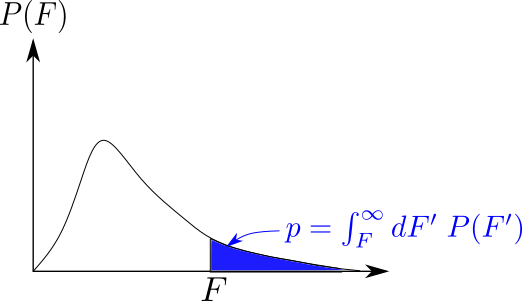
\includegraphics[width=3in]
{ANOVA/f-dist.png}
\caption{Probability distribution $P(F)$
for the F-statistic, 
at fixed $dof_B$ and $dof_W$. See Wikipedia article
Ref.\cite{wiki-f-dist}
for more info about $P(F)$.}
\label{fig-f-dist}
\end{figure}

It's not
hard to find on the Internet, tables 
and 
software calculators 
that give 
the score p-value\footnote{Some tables give
$F=F(p_{sc}, dof_B, dof_W)$
instead of $p_{sc}=p_{sc}(F, dof_B, dof_W)$,
but note that there is a 1-1/onto 
invertible map between $F$ and $p_{sc}$.
Some tables refer  to $p_{sc}$
as $\alp$.
} 
\beq
p_{sc}=\int_{F}^{\infty}
dF'\; P(F'; dof_B, dof_W)
\eeq
of the $F$ statistic,
for a given $dof_B$ and $dof_W$.
See Fig.\ref{fig-f-dist} 
for a portrait of $P(F)$ and $p_{sc}$.
In Bayesian language,
$p_{sc}$
measures
the probability
that $h_0$ is true.
Assume $p_{th}=0.05$.\footnote{
The difference between 
threshold (th)
and score (sc) p-values
is discussed in Section \ref{sec-score-p-value}.}
To determine if the difference between group means is \qt{statistically
significant},
we compare $p_{sc}$ with $p_{th}$. 
If $p_{sc}<p_{th}=0.05$, we reject the null hypothesis.
Otherwise, we fail to reject (accept) the null hypothesis.

If $h_0$ is rejected,  we can  perform {\bf post-hoc} tests to determine how much 
the groups differ from each other.
There are several  popular post-hoc tests,
such as 
the
Tukey test,
Bonferroni test, and 
Scheffe test.

